\chapter{Modèles de saillance}

\section{État de l'art et choix du modèle de saillance}

\par
Il existe aujourd'hui de nombreux modèles de saillance qui permettent de générer des cartes de saillance à partir de scènes naturelles (photos). Le gros avantage de ces modèles est qu'ils permettent d'éviter la fastidieuse tâche de récupération des données oculométriques sur des humains tout en ayant des résultats proches d'une crate de saillance humaine.

\par
Il y a aujourd'hui deux types de modèles de saillance : les modèles "fait-mains", qui appliquent des traitements sur l'image suivant des fonctions mathématiques, et les modèles basés sur l'apprentissage profond, qui s'entrainent sur des bases de données pour s'améliorer. Les modèles fait-mains sont en général plus anciens et précèdent l'avènement du machine learning et de l'apprentissage profond. Ils sont donc généralement moins puissants que les modèles profonds.

\par
Ici notre objectif est de déterminer parmis les modèles qui existent quel est le modèle qui obtient les meilleurs résultats quand on lui donne des peintures en entrée. Pour pouvoir comparer le plus objectivement possible les résultats, il est nécessaire d'utiliser des métriques de qualité. De la même manière que le mètre est utilisé pour mesurer une distance, les métriques sont des outils de mesure avec des échelles variées qui permettent d'associer un score jugeant la qualité de nos cartes de saillances. Il est préférable d'utiliser plusieurs métriques différentes puisque chacune d'entre elles à ses qualités et ses défauts. Ici les métriques utilisées sont celles du benchmark du MIT \cite{benchmark_MIT}.

\par
Mon rôle ici a été de tester tous les modèles profonds pour vérifier dans un premier temps s'il était possible de les faire tourner et dans un second temps de donner des peintures en entrées pour pouvoir y appliquer les métriques de qualité. On peut voir dans l'image \ref{fig:saliencyModel} les résultats des différents modèles comparés à la carte de saillance originale. 

\par
Visuellement il est assez évident de dire que les modèles profonds sont plus proches de la carte de saillance humaine que les autres. Cela se confirme dans l'analyse des métriques. Dans le tableau \ref{tab:scores} on voit que les scores moyens des modèles fait-mains sont tout le temps moins bons que les modèles profonds. Les scores en gras sont les meilleurs scores entre tous les modèles. Ici SAM-ResNet est clairement le plus performant avec le meilleur score dans cinq des sept métriques utilisées. C'est logiquement qu'avec Olivier on a choisi de continuer nos recherches avec SAM-ResNet.

\vfill

\begin{figure}[ht]
    \centering
    \begin{subfigure}{0.24\textwidth}
        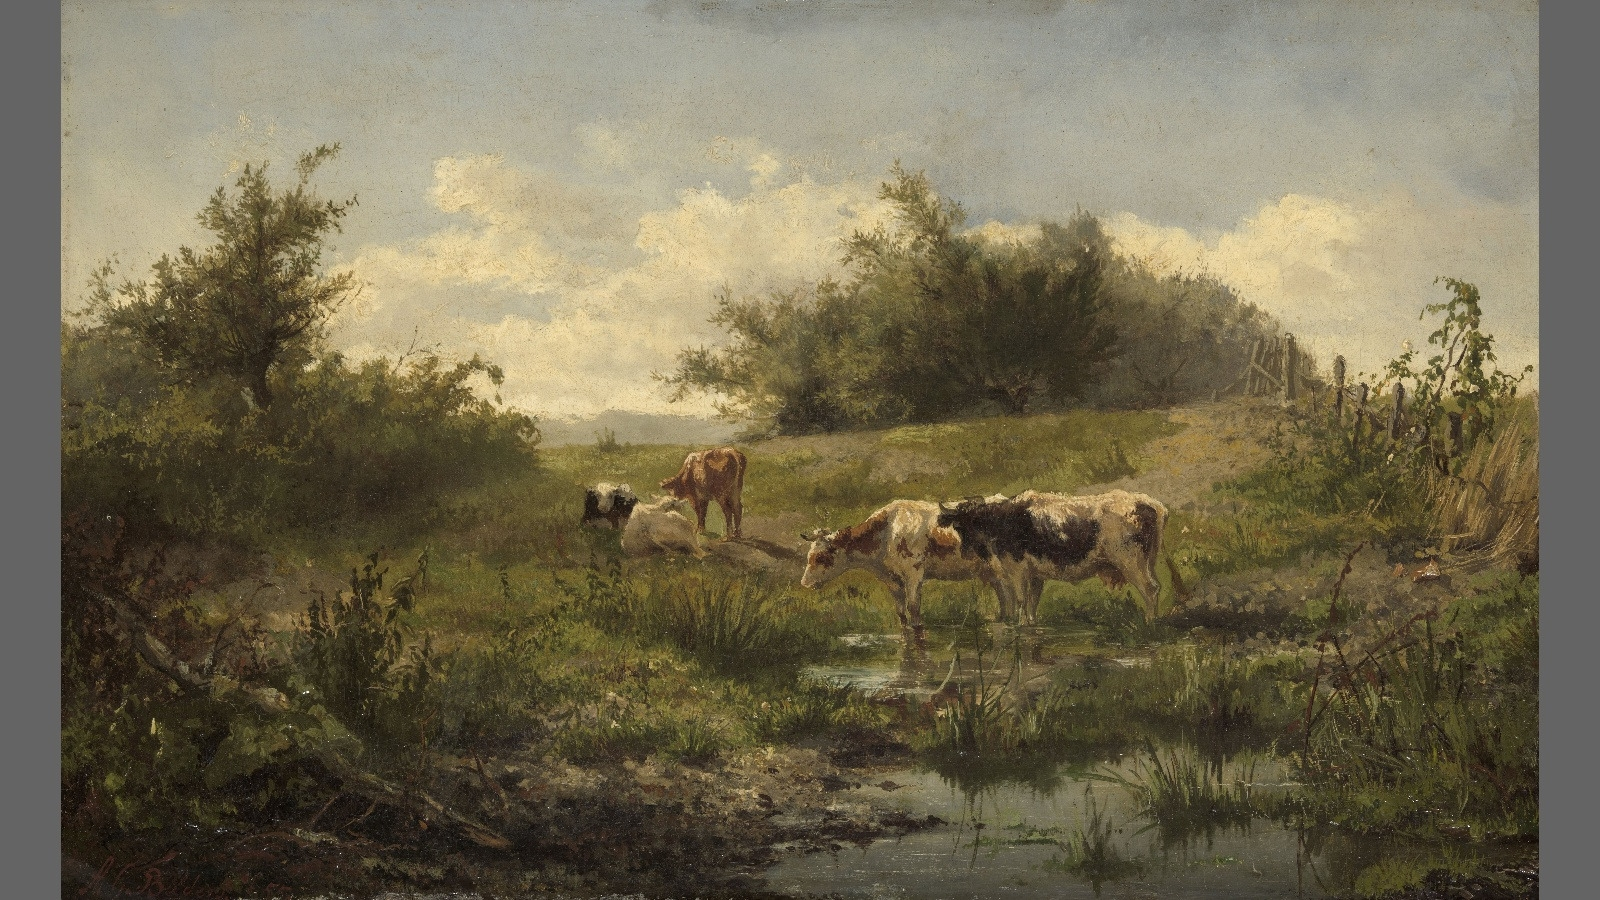
\includegraphics[width=\linewidth]{datas/predictions/stimulus_cows_at_a_pond_Bilders_1856.jpg}
        \caption{}
    \end{subfigure}
    \begin{subfigure}{0.24\textwidth}
        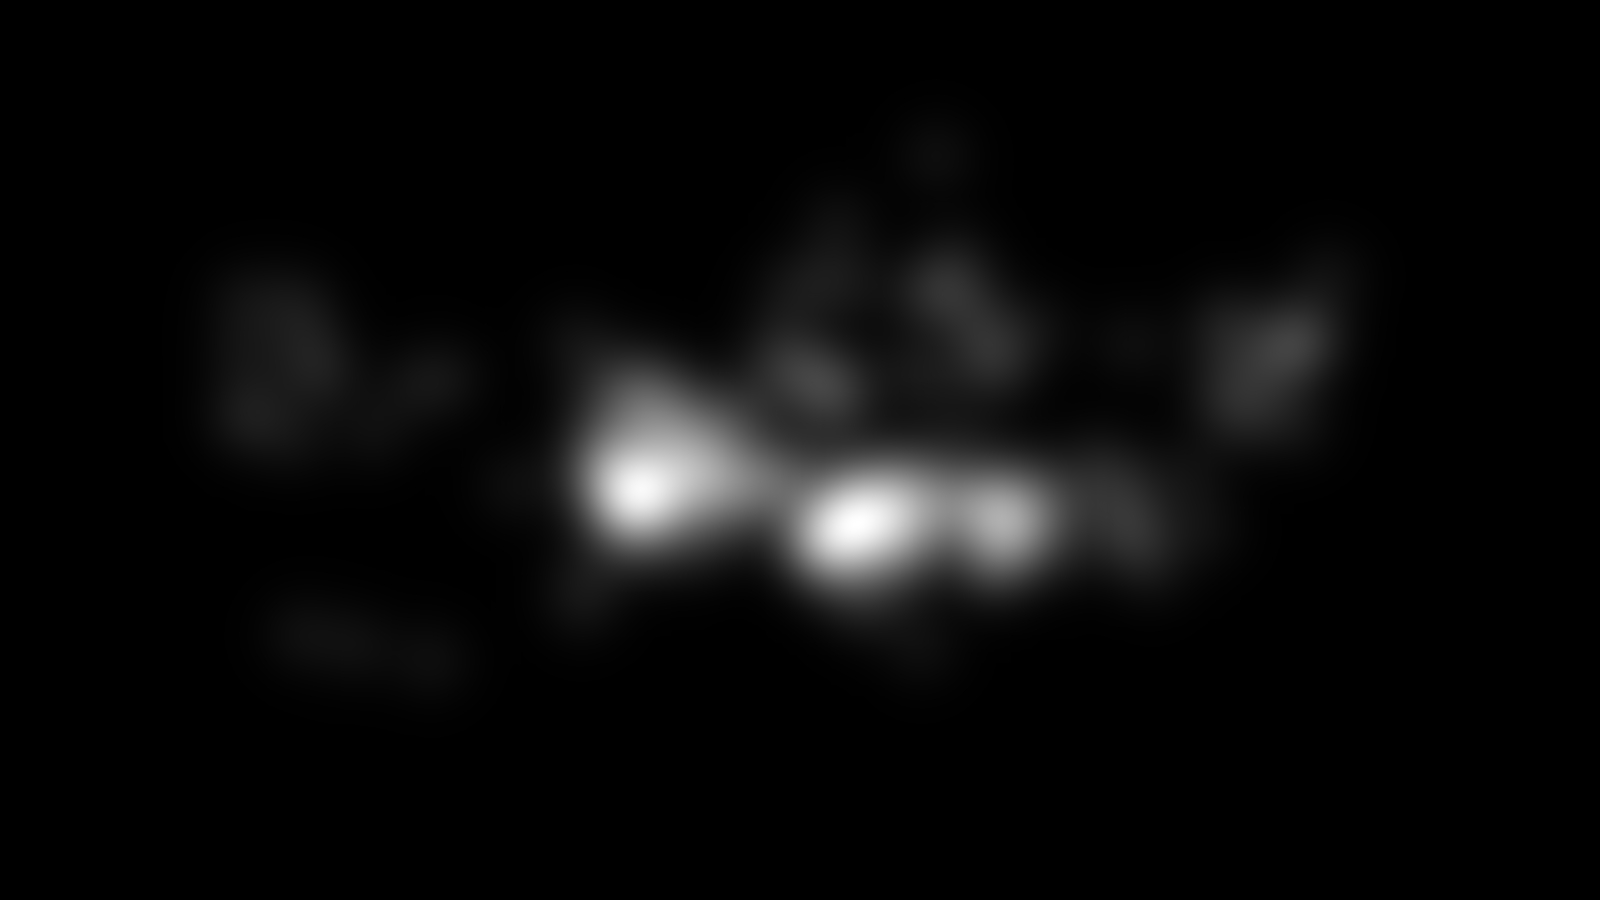
\includegraphics[width=\linewidth]{datas/predictions/human_cows_at_a_pond_Bilders_1856.jpg}
        \caption{}
    \end{subfigure}

    \begin{subfigure}{0.24\textwidth}
        \includegraphics[width=\linewidth]{datas/predictions/gbvs_cows_at_a_pond_Bilders_1856.jpg}
        \caption{GBVS}
    \end{subfigure}
    \begin{subfigure}{0.24\textwidth}
        \includegraphics[width=\linewidth]{datas/predictions/aws_cows_at_a_pond_Bilders_1856.jpg}
        \caption{AWS}
    \end{subfigure}
    \begin{subfigure}{0.24\textwidth}
        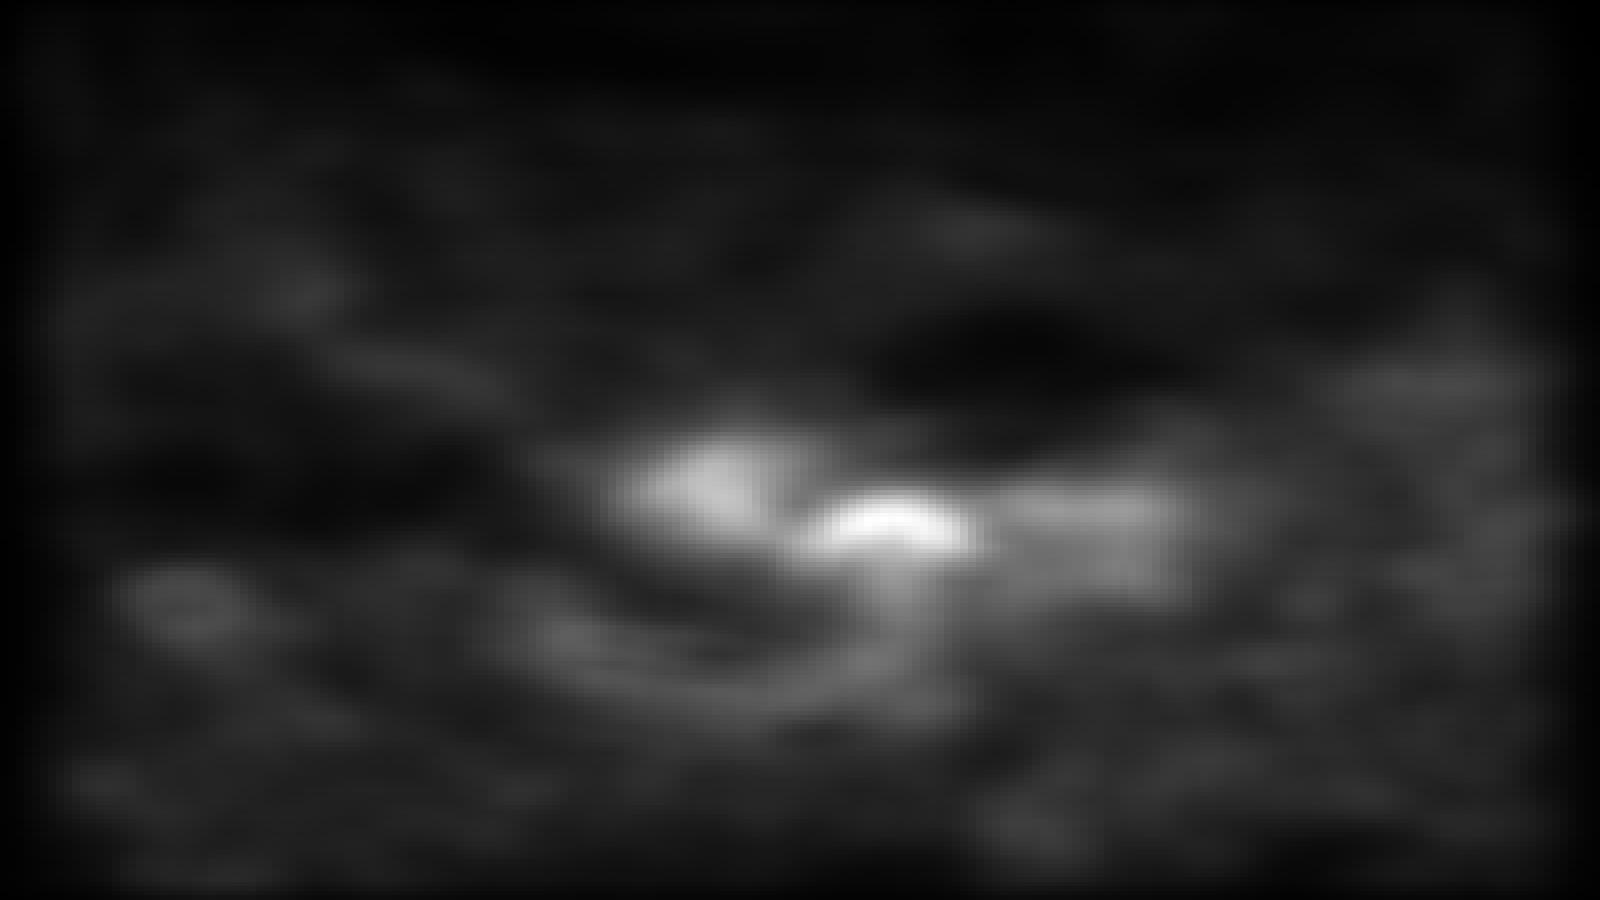
\includegraphics[width=\linewidth]{datas/predictions/rare2012_cows_at_a_pond_Bilders_1856.jpg}
        \caption{RARE2012}
    \end{subfigure}
    \begin{subfigure}{0.24\textwidth}
        \includegraphics[width=\linewidth]{datas/predictions/aim_cows_at_a_pond_Bilders_1856.jpg}
        \caption{AIM}
    \end{subfigure}

    \begin{subfigure}{0.24\textwidth}
        \includegraphics[width=\linewidth]{datas/predictions/mlnet_cows_at_a_pond_Bilders_1856.jpg}
        \caption{MLNET}
    \end{subfigure}
    \begin{subfigure}{0.24\textwidth}
        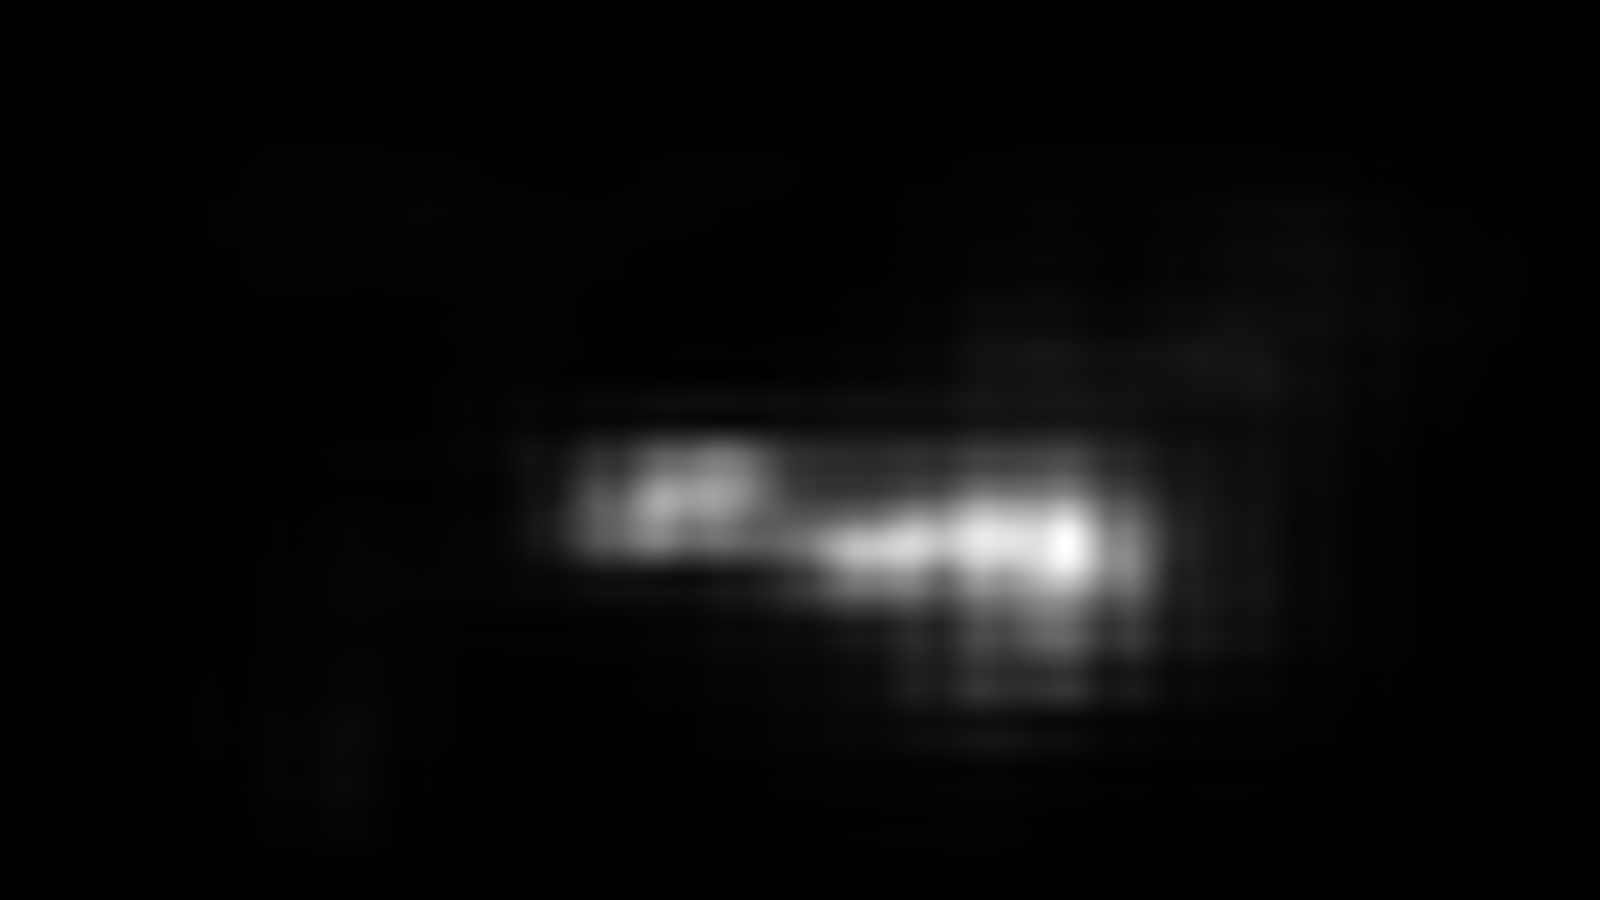
\includegraphics[width=\linewidth]{datas/predictions/SALICON_cows_at_a_pond_Bilders_1856.jpg}
        \caption{SALICON}
    \end{subfigure}
    \begin{subfigure}{0.24\textwidth}
        \includegraphics[width=\linewidth]{datas/predictions/sam_vgg_cows_at_a_pond_Bilders_1856.jpg}
        \caption{SAM-VGG}
    \end{subfigure}
    \begin{subfigure}{0.24\textwidth}
        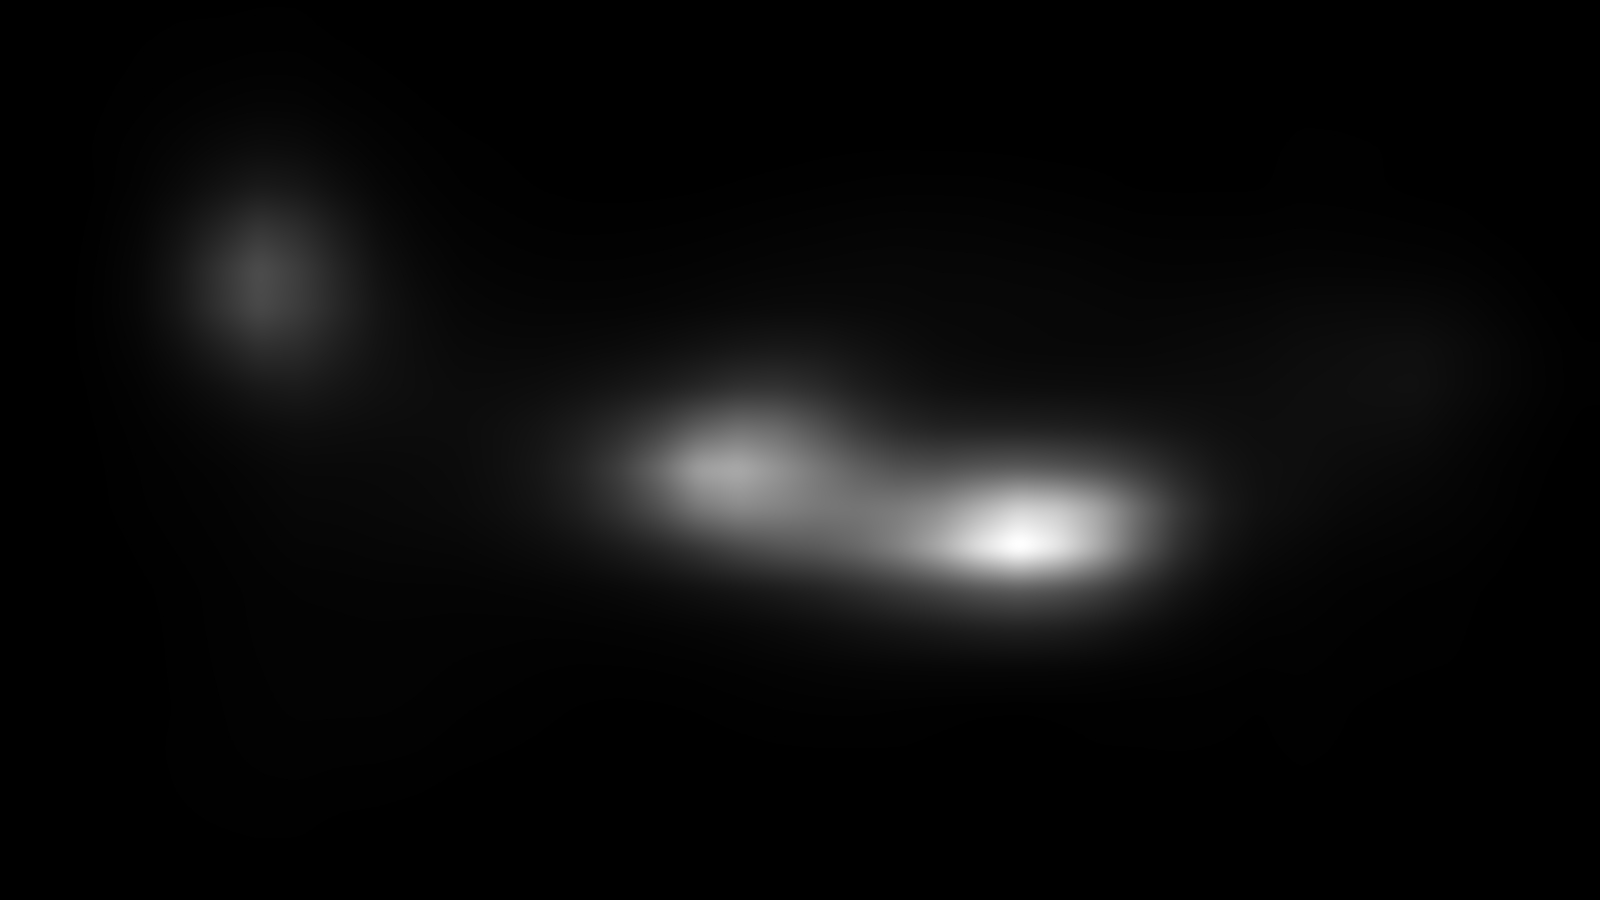
\includegraphics[width=\linewidth]{datas/predictions/sam_resnet_cows_at_a_pond_Bilders_1856.jpg}
        \caption{SAM-ResNet}
    \end{subfigure}
     
    \caption{Cartes de saillance de modèles fait-mains (2\up{ème} ligne) et profonds (3\up{ème} ligne). La 1\up{ère} ligne illustre le stimuli originale et sa carte de saillance humaine}
    \label{fig:saliencyModel}
\end{figure}

\vfill

\begin{table}[ht]
    \centering
        \begin{tabular}{|l|l|l|l|l|l|l|}
		\hline
        Modèle & CC~$\uparrow$ & KL~$\downarrow$ & SIM~$\uparrow$ & NSS~$\uparrow$ & AUC-B~$\uparrow$ & AUC-J~$\uparrow$\\
		\hline
        GBVS        & 0.506 & 0.962 & 0.446 & 1.256 & \textbf{0.809} & 0.817\\
        RARE2012    & 0.443 & 1.020 & 0.438 & 1.103 & 0.777 & 0.786\\
        AIM         & 0.315 & 1.245 & 0.371 & 0.772 & 0.723 & 0.735\\
        AWS         & 0.427 & 1.045 & 0.430 & 1.083 & 0.762 & 0.769\\
		\hline
        Moyenne     & 0.422 & 1.068 & 0.421 & 1.053 & 0.774 & 0.776\\
		\hline
        MLNET       & 0.576 & \textbf{0.832} & 0.513 & 1.524 & 0.770 & 0.818\\
        DeepGazeII  & 0.485 & 0.896 & 0.488 & 1.394 & 0.679 & 0.804\\
        SALICON     & 0.538 & 0.880 & 0.517 & 1.445 & 0.708 & 0.827\\
        SAM ResNet  & \textbf{0.700} & 0.984 & \textbf{0.613} & \textbf{1.834} & 0.782 & \textbf{0.862}\\
        SAM VGG     & 0.617 & 0.970 & 0.561 & 1.603 & 0.752 & 0.846\\
		\hline
        Moyenne     & 0.583 & 0.912 & 0.551 & 1.560 & 0.738 & 0.831\\
		\hline
        \end{tabular}
    \caption{Performances des modèles de saillance sur les peintures de la base de données.}
    \label{tab:scores}
\end{table}

\vfill

\newpage
\section{Entrainement du modèle}

\par
On a donc un modèle profond pré-entrainé pour déterminer la saillance dans les scènes naturelles. Pour adapter ce modèle aux peintures afin d'obtenir de meilleurs scores et donc une meilleure qualité dans les cartes de saillance générées, on va faire du "\textbf{fine tuning}" que l'on peut traduire par "ajustement". C'est-à-dire qu'au lieu d'entrainer le modèle en partant de zéro, on va prendre les poids du modèle actuel et entrainer le modèle à partir de ceux-ci. Si on compare ça a une course, au lieu de commencer la course au départ, on part d'un checkpoint au milieu de la course. Cela permet de gagner du temps lors de l'entrainement sans perdre en qualité.

\par
La base de données utilisée pour l'entrainement est celle décrite dans la partie \ref{database}. Des 150 peintures disponibles, 90 sont utilisées pour l'entrainement, 20 pour la validation et les 40 dernières sont pour le test du modèle. Les peintures étaient dans un premier temps choisies par ordre alphabétique, ce qui était supposément un ordre aléatoire. Il s'est avéré après coup que la plupart des natures mortes ou des peintures nues avait le genre dans leur titre ce qui faussait l'aléatoire. J'ai donc créer un petit script qui m'as permis de faire la séparation de ma base de données de manière complètement aléatoire. Cela a permis d'améliorer la qualité des cartes de saillance générées.

\begin{table}[ht]
    \centering
    \begin{tabular}{|l|l|l|l|l|l|l|}
        \hline
        Modèle & CC~$\uparrow$ & KL~$\downarrow$ & SIM~$\uparrow$ & NSS~$\uparrow$ & AUC-B~$\uparrow$ & AUC-J~$\uparrow$\\
        \hline
        SAM ResNet              & 0.691 & 1.088 & 0.609 & 1.792 & 0.786 & 0.857\\
        SAM ResNet (fine-tuné)  & 0.758 & 0.836 & 0.681 & 1.922 & 0.845 & 0.882\\
        \hline
        Gain (\%)               & +9.7\% & -23\% & +11.8\% & +7.2\% & +7.5\% & +2.9\%\\
        \hline
    \end{tabular}
    \caption{Performances de SAM-ResNet après fine-tuning}
    \label{tab:scoresfinetuned}
\end{table}

\par
Les résultats obtenus après l'entrainement sont plutôt bons. Les scores avant et après des métriques sont visibles dans le tableau \ref{tab:scoresfinetuned}. Toutes les métriques montrent un score supérieur pour le modèle ré-entrainé. Un exemple des résultats sur les images \ref{fig:avantapres} montre qu'effectivement sans être une copie conforme de la carte de saillance humaine, la version ré-entrainée de Sam-ResNet donne des résultats corrects.

\begin{figure}[ht]
    \centering
    \begin{subfigure}{.49\textwidth}
        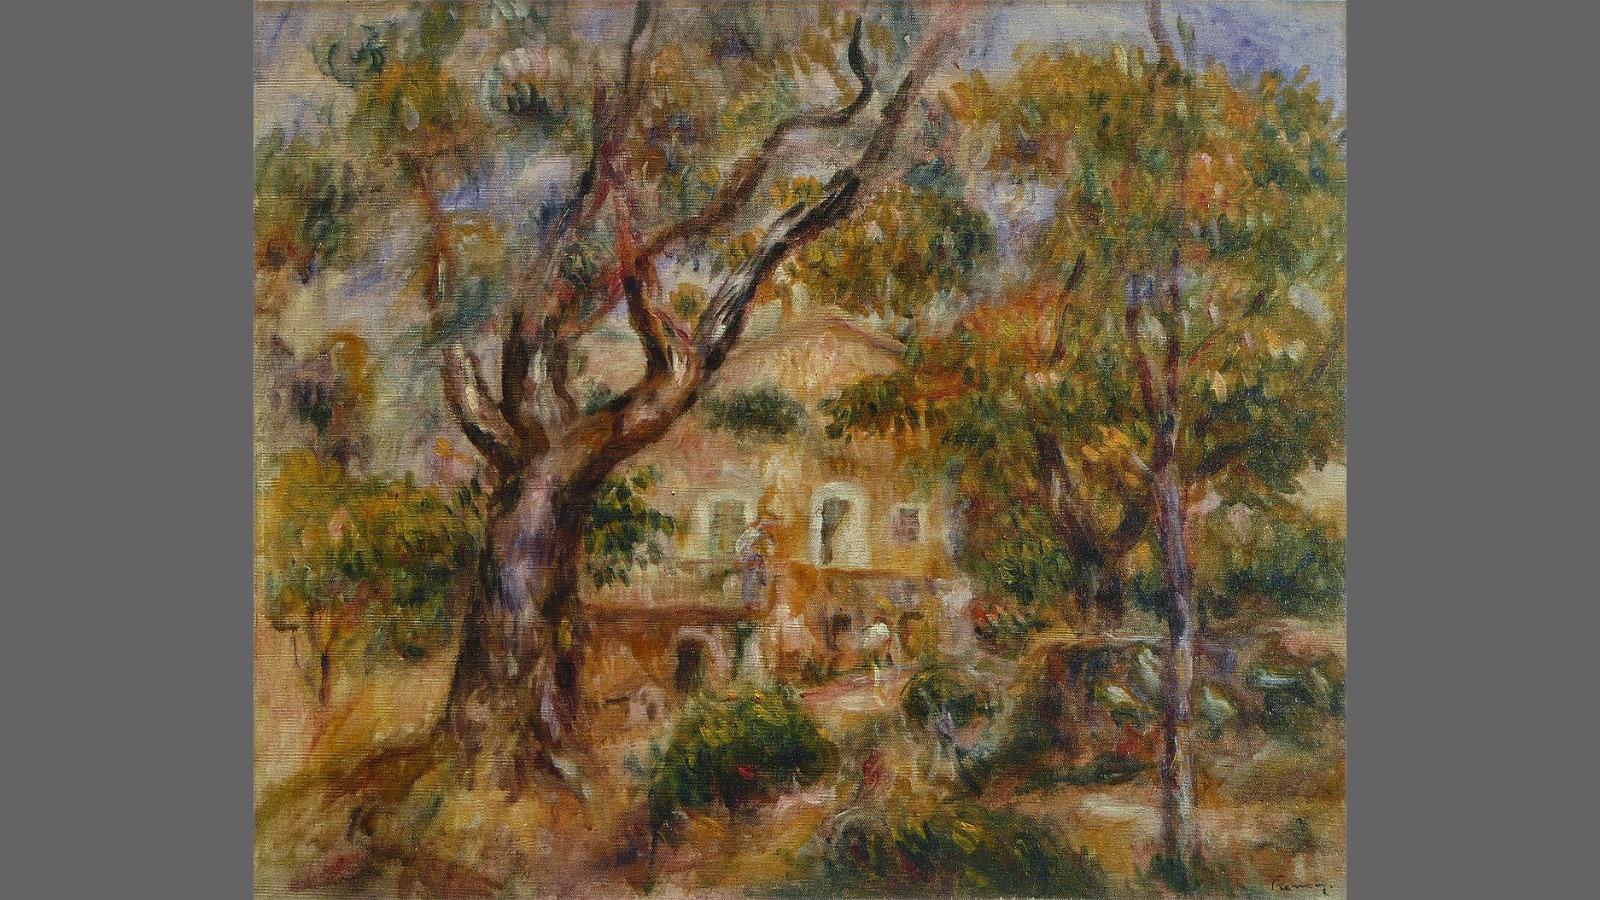
\includegraphics[width=\linewidth]{datas/samresnet/stimulus_La_Ferme_des_Collettes_Renoir_1908.png}
        \caption{}
    \end{subfigure}
    \begin{subfigure}{.49\textwidth}
        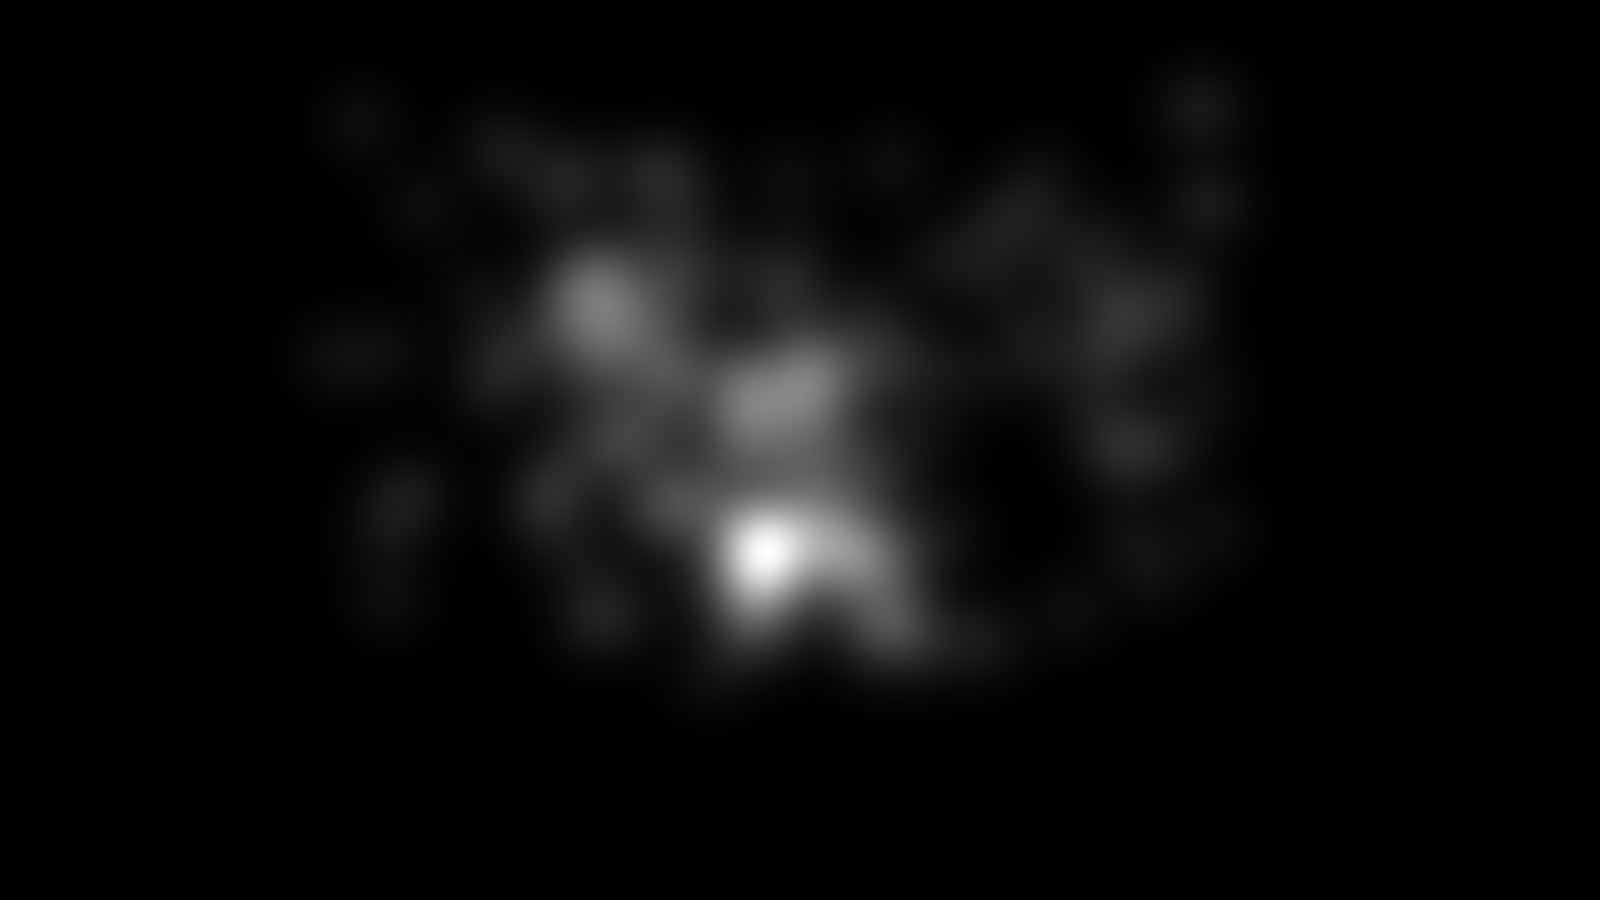
\includegraphics[width=\linewidth]{datas/samresnet/human_La_Ferme_des_Collettes_Renoir_1908.png}
        \caption{}
    \end{subfigure}

    \begin{subfigure}{.49\textwidth}
        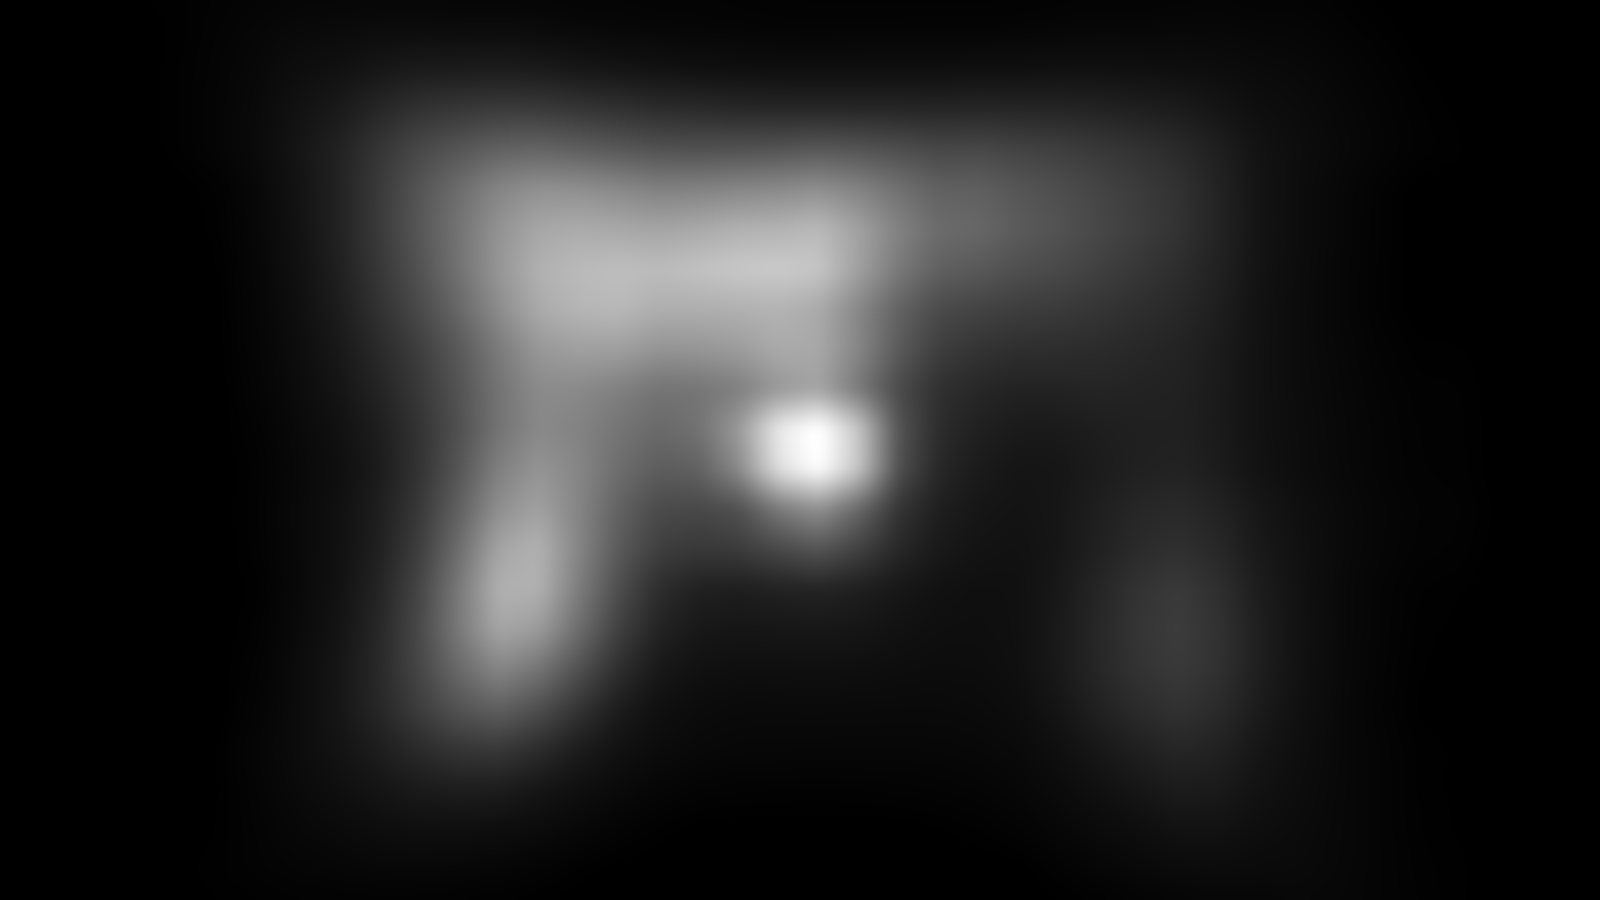
\includegraphics[width=\linewidth]{datas/samresnet/orig_La_Ferme_des_Collettes_Renoir_1908.png}
        \caption{}
    \end{subfigure}
    \begin{subfigure}{.49\textwidth}
        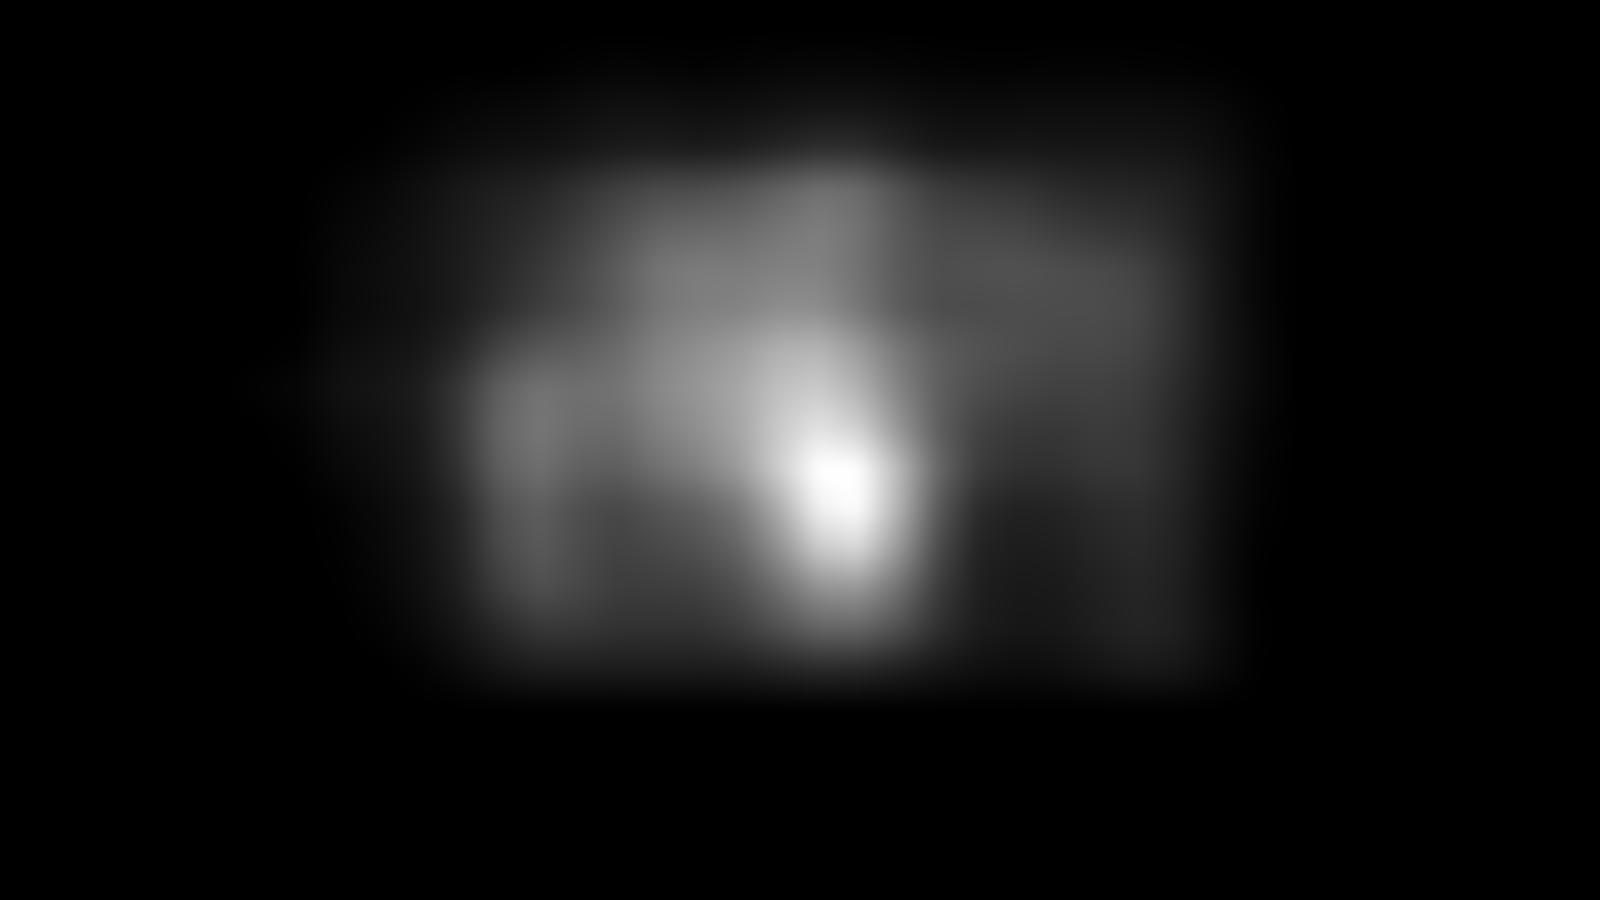
\includegraphics[width=\linewidth]{datas/samresnet/retrain_La_Ferme_des_Collettes_Renoir_1908.png}
        \caption{}
    \end{subfigure}
    \caption{(a) Peinture originale, (b) carte de saillance humaine, (c) prédiction SAM-ResNet et (d) prédiction de SAM-ResNet ré-entrainé . (Renoir, La ferme des Collettes, 1908.)}
    \label{fig:avantapres}
\end{figure}

\par
Cependant il est important de noté que les mouvements artistiques des peintures influencent le résultat du modèle de saillance. En effet les résultats sont bien meilleurs sur des peintures appartenant au mouvement du Réalisme ou du Romantisme que celles du Pointillisme ou de l'Impressionisme. Cela est dû au fait que le modèle étant construit et entrainé originellement pour des scènes naturelles est ce qui se rapproche le plus des peintures réalistes. Pour améliorer les résultats je pense qu'il faudrait ré-entrainer entièrement le modèle avec une plus grande base de données et avoir plus de diversité avec plus de styles et de mouvements différents.